\documentclass[notoc, landscape]{school}
\title{RAW Import und einfache Retusche}
\subject{Medientechnik - Fotografie}
\author{Markus Reichl}

\begin{document}
\thispagestyle{fancy}

Die folgende Anleitung beschäftigt sich mit dem Import von RAW\cite{wiki-raw} Aufnahmen und der anschließenden Bearbeitung in Adobe Photoshop oder Lightroom CC.

\section{RAW Import}
\begin{multicols}{2}
\begin{outline}[enumerate]
\1 Rohdaten Datei anwählen und via Rechtsklick \texttt{Öffnen mit} und \texttt{Photoshop} / \texttt{Lightroom} anwählen.

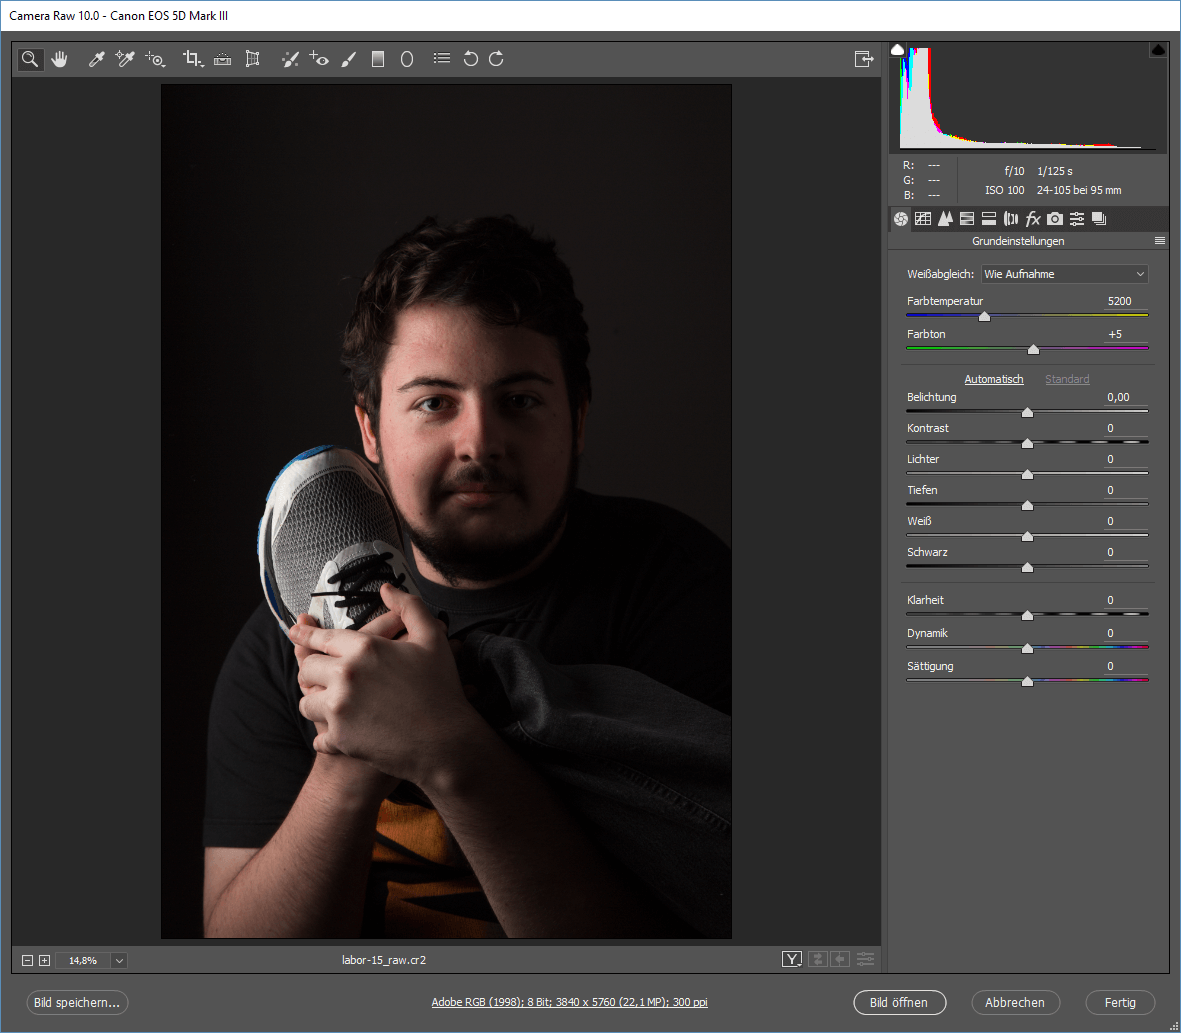
\includegraphics[width=10cm]{raw-01.png}

\columnbreak

\1 Gewünschte Änderungen vornehmen. Mögliche Ansätze:
	\2 \texttt{Grundeinstellungen} Einstellung von Weißabgleich, Farbsättigung und Tonwertbereich.

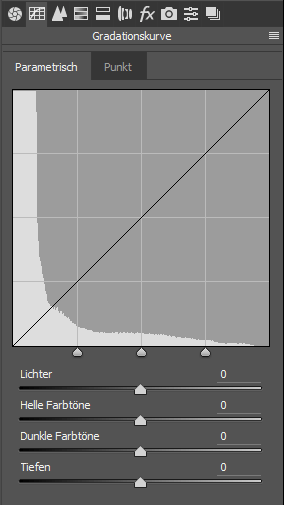
\includegraphics[height=6cm]{raw-03-grad.png}
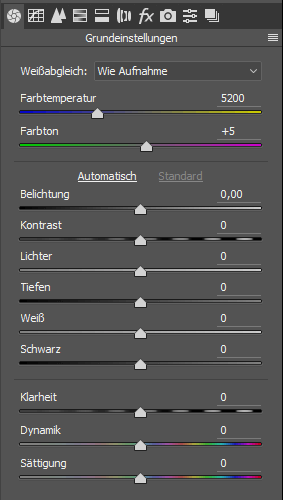
\includegraphics[height=6cm]{raw-02-grund.png}

	\2 \texttt{Gradationskurve} Optimierung von Tonwerten mithilfe der parametrischen Kurve.

\1 Im Dialogfeld \texttt{Camera Raw} die Datei im gewünschten Format\footnote{Digital Negative (DNG), JPEG, TIFF oder PSD (Photoshop)} speichern.\footnote{\begin{quote}"Mit der Software Photoshop Camera Raw kann eine Bilddatei mit Rohdaten zwar geöffnet und bearbeitet, aber nicht in einem Rohdatenformat gespeichert werden."\end{quote}\cite{adobe-raw}}

Eine detaillierte Anleitung findet sich auf der Adobe Help Board Website\cite{adobe-raw}.
\end{outline}
\end{multicols}

\newpage
\section{Einfache Retusche}
\begin{minipage}{.65\textwidth}
\begin{outline}[enumerate]
\1 Datei anwählen und via Rechtsklick \texttt{Öffnen mit} und \texttt{Photoshop} / \texttt{Lightroom} anwählen.
\1 Es empfiehlt sich bereits zu Beginn die Hintergrund Ebene zu duplizieren um eine zerstörungsfreie Bearbeitung durchzuführen.
\begin{center}
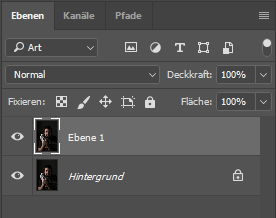
\includegraphics[height=3cm]{retusche-01-ebene.png}
\end{center}
\1 Bei Aufnahmen von geringerer Qualität können vor Beginn der eigentlichen Bearbeitung die Farbtonkorrekturen automatisch durchführen zu lassen.
	\2 \texttt{Ebene > Neue Einstellungsebene > Tonwertkorrektur} / \texttt{Gradationskurven} anwählen.
	\2 Im \texttt{Eigenschaftenbedienfeld} \texttt{Auto} anwählen.
	\2 Im Dialogfeld \texttt{Auto-Farbkorrekturoptionen > Algorithmen > Schwarzweiß-Kontrast verbessern} können zu beschneidende Tiefen und Lichter festgelegt werden.
	\2 Mit \texttt{Ok} werden die Änderungen angewandt.
\end{outline}
\end{minipage}
\begin{minipage}{.35\textwidth}~\\\\\\
\begin{center}
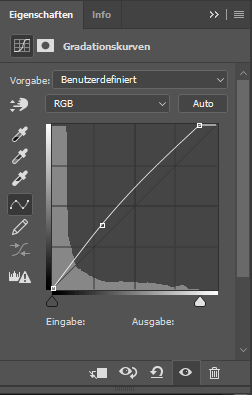
\includegraphics[height=6cm]{retusche-02-grad.png}
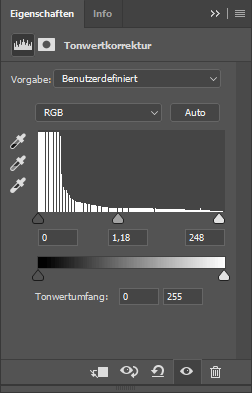
\includegraphics[height=6cm]{retusche-03-tonwert.png}
\end{center}
\end{minipage}
\vfill
Eine detaillierte Anleitung findet sich auf der Adobe Help Board Website\cite{adobe-quick-adjustments}.
\newpage
\subsection{Haut}
\begin{outline}[enumerate]
\1 Hautunreinheiten und unerwünschte Stellen können mit dem \texttt{Ausbessern} Werkzeug entfernt werden.
	\2 Zu Beginn empfiehlt es sich die Stellen hervorzuheben.
		\3 \texttt{Ebene > Kanalmixer} anwählen und im Menü \texttt{Vorlagen} die Option\\\texttt{Schwarzweiß-Infrarot} anwählen.
			\4 Oder \texttt{Kanalmixer > Filter > Rauschfilter > Helligkeit interpolieren} anwählen.

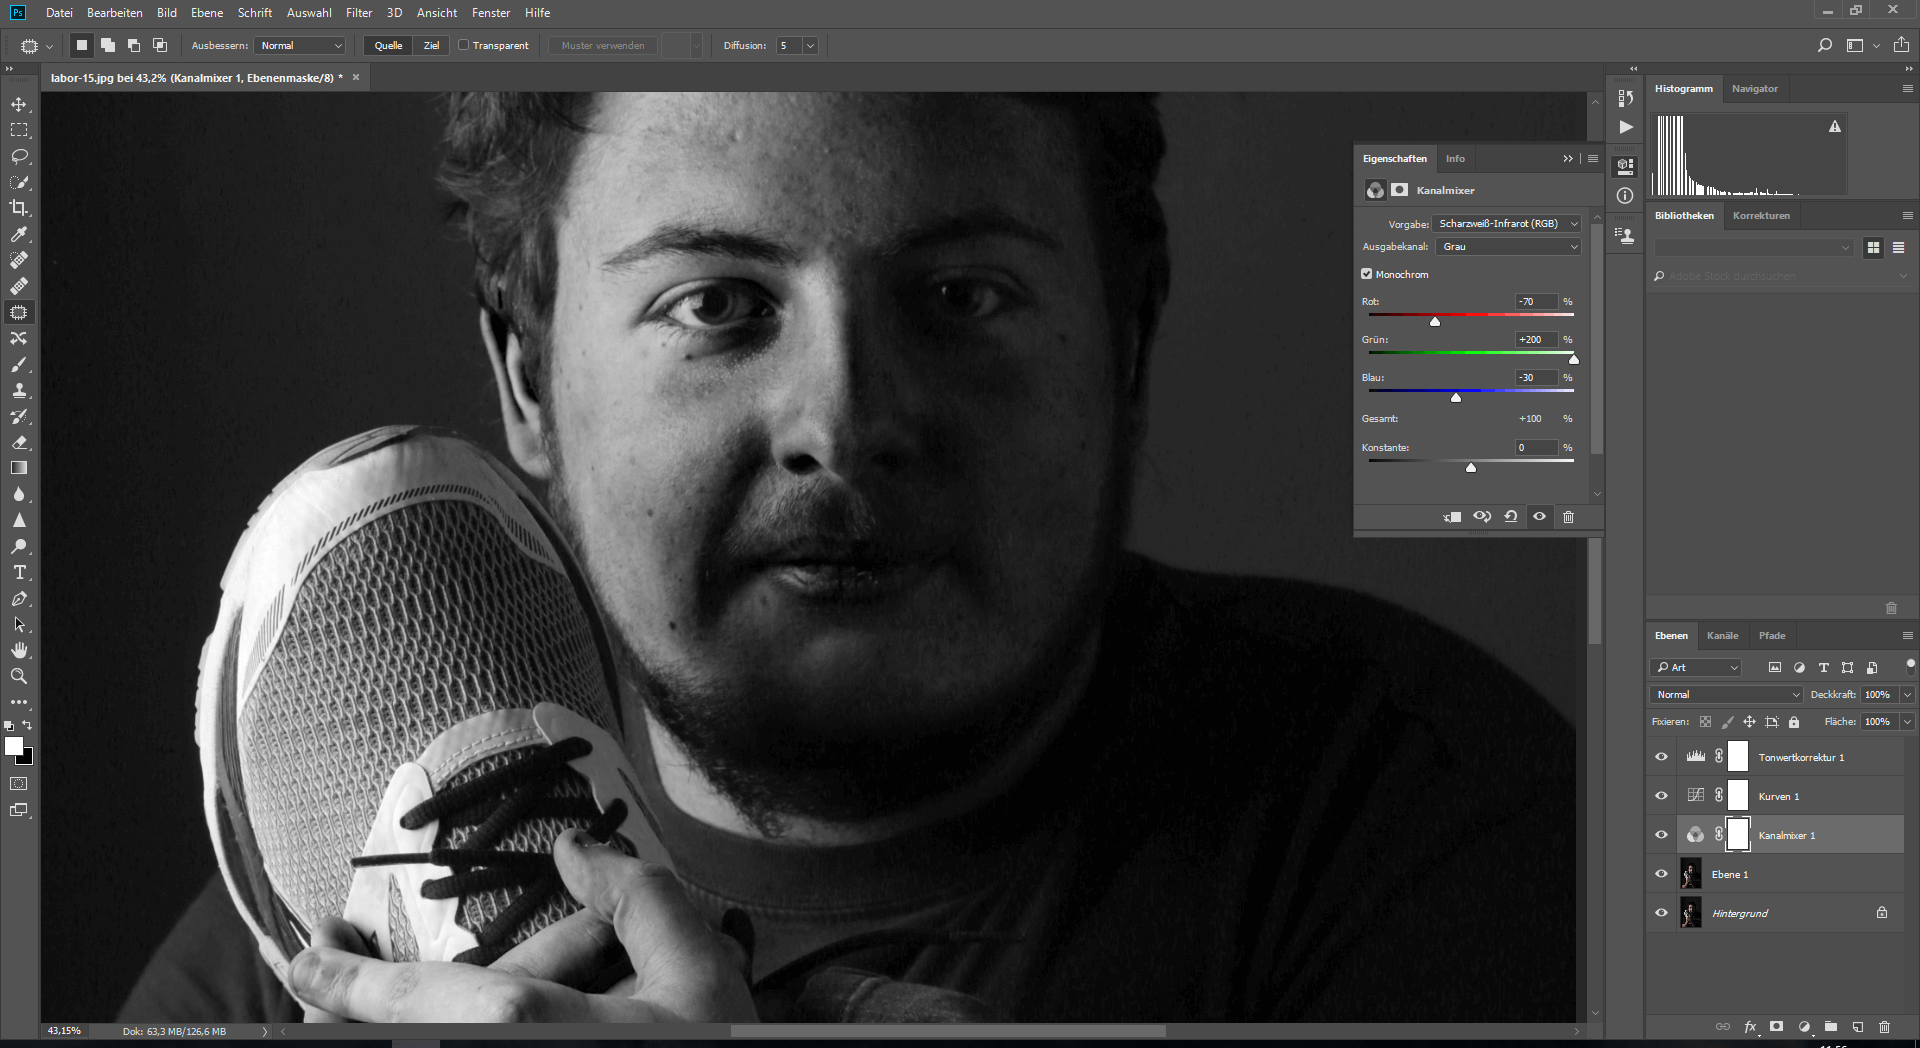
\includegraphics[height=8cm]{retusche-04-kanalmixer.png}

		\3 Farbliche Unebenheiten werden sehr dunkel dargestellt und Umrisse sind leicht erkennbar.
	\newpage
	\2 Unerwünschte Stellen können nun entfernt werden. Dazu empfiehlt es sich eine neue Ebene zu erstellen.
		\3 Mit dem \texttt{Ausbessern} Werkzeug eine Stelle markieren (die Funktion ist mit der des \texttt{Auswahl} Werkzeugs ident).

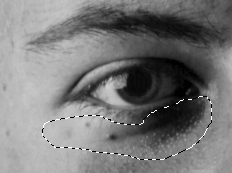
\includegraphics[height=3cm]{retusche-05-auswahl.png}

		\3 Innerhalb der Auswahl den Inhalt "verschieben" bis der Bereich innen, dem gewünschten Ergebnis entspricht.

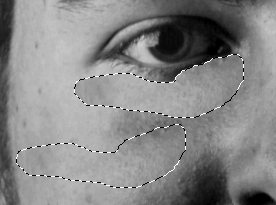
\includegraphics[height=4cm]{retusche-06-verbesserung.png}
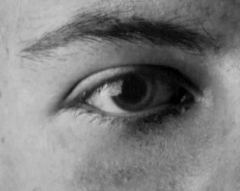
\includegraphics[height=3cm]{retusche-07-verbessert.png}

		\3 Vorgang für alle weiteren Stellen wiederholen.
	\newpage
	\2 Zuletzt kann die Haut noch Weichgezeichnet werden um kollektiv Unebenheiten zu entfernen. Dazu kann theoretisch eine beliebige Weichzeichnungsmethodik verwendet werden, empfohlen wird dabei die Funktion \texttt{Filter > Weichzeichnungsfilter > Selektiver Weichzeichner}.

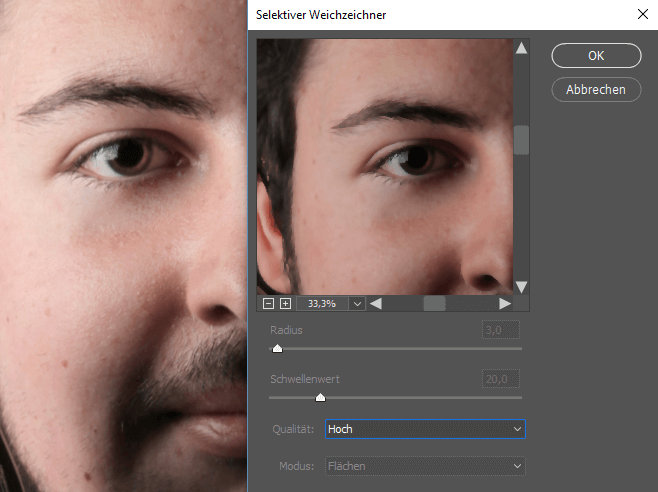
\includegraphics[height=6cm]{retusche-08-weich.png}

\1 
Damit ist die grundlegende Retusche beendet. Als weiterer Schritt empfiehlt sich die Anpassung der Farbe durch Einstellebenen wie 2 \texttt{Ebene > Neue Einstellungsebene > Tonwertkorrektur} oder \texttt{Ebene > Neue Einstellungsebene > Gradationskurven}. Detailliertere Anleitungen finden sich auf der Adobe Help Board Website\cite{adobe-levels}\cite{adobe-curves}.
\end{outline}

\begin{thebibliography}{9}

% \bibitem{faz} faz.net, Vergewaltigung live auf Facebook gezeigt \\ http://www.faz.net/aktuell/gesellschaft/kriminalitaet/vergewaltigung-live-auf-facebook-gezeigt-14936872.html
\bibitem{wiki-raw} Wikipedia, Rohdatenformat \\ https://de.wikipedia.org/wiki/Rohdatenformat
\bibitem{adobe-raw} Adobe Help Board, Einführung in Camera RAW \\ https://helpx.adobe.com/at/camera-raw/using/introduction-camera-raw.html
\bibitem{adobe-quick-adjustments} Adobe Help Board, Durchführung schneller Farbtonkorrekturen \\ https://helpx.adobe.com/de/photoshop/using/making-quick-tonal-adjustments.html
\bibitem{adobe-blur} Adobe Help Board, Anpassen der Bildschärfe \\ https://helpx.adobe.com/de/photoshop/using/adjusting-image-sharpness-blur.html
\bibitem{adobe-levels} Adobe Help Board, Verwenden der Tonwertkorrektur \\ https://helpx.adobe.com/de/photoshop/using/levels-adjustment.html
\bibitem{adobe-curves} Adobe Help Board, Verwenden der Gradationskurven \\ https://helpx.adobe.com/de/photoshop/using/curves-adjustment.html

\end{thebibliography}
\end{document}